%%\documentclass[11pt,twocolumn]{report}
\documentclass[10pt]{article}

\usepackage{hyperref}
\usepackage{array}
\usepackage{graphicx}
\usepackage{float}
\usepackage[procnames]{listings}
\usepackage{color}
\usepackage[square,sort,comma,numbers]{natbib}
\usepackage[bottom]{footmisc}
\usepackage{pdfpages}
\usepackage{fullpage}
\usepackage{hyperref}
\usepackage{epstopdf}


\renewcommand{\bibsection}{}

\newfloat{listing}{H}{lop}
\floatname{listing}{Listing}



%%\renewcommand{\bibname}{References} 
\newcommand{\q}[1]{``#1''}
\newcommand{\HRule}{\rule{\linewidth}{0.5mm}}


%\title{Research Project 1 - Monitoring DNSSEC}

%\author{
%	Martin Leucht \\ 
%	\texttt{martin.leucht@os3.nl}
%	\and Julien Nyczak \\
%	\texttt{julien.nyczak@os3.nl}
%	\and Supervisor: Rick van Rein
%	\and 
%	\and 
%	\and System and Network Engineering
%	\and University of Amsterdam
%}




%%\renewcommand*\contentsname{Table of Contents}

\begin{document}
\definecolor{keywords}{RGB}{255,0,90}
\definecolor{comments}{RGB}{0,0,113}
\definecolor{red}{RGB}{160,0,0}
\definecolor{green}{RGB}{0,150,0}
 
\lstset{language=Python, 
        basicstyle=\ttfamily\tiny, 
        keywordstyle=\color{keywords},
        commentstyle=\color{comments},
        stringstyle=\color{red},
        showstringspaces=false,
        identifierstyle=\color{green},
        procnamekeys={def,class}}
%%\maketitle
\input{Front_page.tex}

\thispagestyle{empty}
\newpage

\begin{abstract}
Monitoring DNSSEC zones is essential to keep them fully operational. Although SNMP is a very old fashioned protocol, it is still widely used to monitor devices on IP Networks and can be implemented for applications as well, such as DNSSEC. This paper focuses on building a proof of concept for monitoring DNSSEC through SNMP. To that aim, we have constructed an SNMP MIB module that, once loaded to an SNMP subagent, provides DNSSEC critical parameters to a monitoring station. DNSSEC data is retrieved periodically by Python scripts and inserted into a central XML file parsed by the SNMP subagent. New zones are handled automatically when simply specified in a configuration file. The usage of SNMP makes our proof of concept easily deployable. However, it lacks features such as notifications and might show performance issues when it comes to monitor a large number of zones.
\end{abstract}

\newpage

\tableofcontents

\newpage

\section{Introduction}
\label{chap:introduction}
As figures demonstrate, DNSSEC (Domain Name System Security Extension) becomes more and more popular. Indeed, 77\% of top-level domains (TLDs) have trust anchors published as delegation signer (DS) records in the root zone\cite{stats}. However, to function properly, resource records (RR) of a DNSSEC-enabled zone need to be regularly signed since signatures have an expiration date. If signatures have not been refreshed in time, the zone becomes unreachable. This is not acceptable.
\\
Monitoring DNSSEC parameters, such as signature expiration dates, could avoid those undesired effects. For instance, a monitoring system would send notifications to the zone maintainer when a resource record signature (RRSIG) of a resource record is about to expire.
\\
There exist a lot of approaches to monitor DNSSEC. For example, service providers offering DNSSEC services have developed their own utilities, often strongly related to their infrastructures and demands. None of these solutions uses the Simple Network Management Protocol (SNMP). SNMP provides an abstraction model for data required to be monitored. This data is represented in a common format, known as an SNMP Management Information Base (MIB). Thus, it makes it applicable for a generic use in monitoring systems, rather than for custom made solutions. The absence of a MIB module for DNSSEC urges to develop such a solution.

\subsection{Related Work}
As pointed out earlier, there are plenty of monitoring systems already existing for DNSSEC\cite{list}, but we are looking for an integrated SNMP-compliant tool. We want to write our SNMP sub-agent in Python, and some work has already been done towards that direction. Indeed, \textit{python-netsnmpagent}\cite{pythonnetsnmpagent} is a Python module that facilitates the writing of Net-SNMP subagents in Python.
Furthermore, a DNS server MIB\cite{dnsmib} has already been created. Its purpose was to manage DNS name server (e.g. updating zones) but has been retired since\cite{dnsmib_retire} because inter alia, goals were not clearly defined. However, MIB modules for DNSSEC monitoring do not seem to have ever been created.


\subsection{Research Questions}
Our main goal is to develop an SNMP-compliant monitoring prototype solution. This implies the definition of a set of variables meaningful to the well-being of a DNSSEC signed zone, the construction of a MIB module for DNSSEC, and the development of an SNMP agent meant to feed the MIB. This naturally leads to the following research questions.
\begin{itemize}
\item What are vital life signs for monitoring DNSSEC?
\item How to construct a MIB module for DNSSEC?
\item How to conduct monitoring based on such a MIB?
\item How do architectures for monitoring DNSSEC compare?
\end{itemize}

\newpage

\section{Background}
\label{chap:background}
\subsection{SNMP}
SNMP is a de facto standard application protocol to manage and monitor devices running on IP networks and is defined in several RFC's \cite{snmp-rfc}. SNMP is a connectionless protocol using UDP Port 161. SNMP provides an abstract interface to serve status information about IP capable devices or applications to a management station. Classical candidates that support SNMP are network devices such as routers and switches. SNMP can also be implemented on Operating Systems or application extensions. Version 3 of the SNMP protocol includes authentication, privacy, and access control \cite{cisco-snmp}.  
\\
SNMP provides an agent-manager architecture. The agent facilitates an SNMP interface that allows a manager to get (or sometimes set) management information data from a managed device in an SNMP-specific form. An agent can be implemented as a subagent that registers data to a master agent by using the AgentX protocol \cite{agentx}. The structure of the management information and available SNMP variables are defined in a Management Information Base (MIB) which follows strict syntax rules defined in the Structure of Management Information Version 2 (SMIv2) \cite{smiv2}. SMIv2 is a subset of ASN.1. 
\\
SNMP variables are assigned to Object Identifiers (OID) and organized in a hierarchical structure. Before writing an SNMP MIB, an OID entry point inside the global MIB tree has to be defined. Those entry points are located under the internet branch \cite{oid1}. Public branches  inside the mgmt subtree are defined by the Internet Engineering Task Force (IETF). Private branches inside the private subtree are assigned to companies by the Internet Assigned Numbers Authority (IANA). An OID requires to be unique to avoid overlapping with other MIBs. For testing purposes an experimental subtree exists. 

\subsection{DNSSEC}
DNS stands for Domain Name System. It is a decentralized hierarchical distributed system that mainly translates domain names to IP addresses. As DNS does not provide integrity nor authentication, DNS data can be subject to forgery. Hence, DNSSEC has been specified to solve this problem. It uses public key cryptography and cryptographically signs the resource records of a zone so a chain of trust can be build from the root down.
To understand the concept of this chain of trust, let's walk it from bottom up, with \textit{derby.os3.nl.} as a zone example. 
\\
First of all, the \textit{derby.os3.nl.} zone must have at least two (for key management simplification) key-pairs published in the DNS, a Key Signing Key (KSK) and a Zone Signing Key (ZSK). They form the DNSKEY RRset of the zone. The ZSK is used to sign all the resource records in a zone. It is usually 1024 bits long and is rolled-over more often than a KSK (every two weeks is common practise). The main reason for key-rollovers is the fact that the longer a key is published, the higher is the probability that the key gets compromised by an attacker. A KSK is meant to validate the DNSKEY RRset. Since it is supposed to be rolled-over less frequently than a ZSK, it is obvious that its size is bigger (most often 2048 bits). In addition, the KSK needs to be validated as well. To that end, the hash of the public key is published in the parent zone (\textit{os3.nl.} in our example) as a DS record. In other words, the KSK acts a Secure Entry Point (SEP) from the zone \textit{os3.nl.} to \textit{derby.os3.nl.}. Next, the same validation process occurs for the \textit{os3.nl.} zone, then for the \textit{nl.} zone to  finally reach the root zone. Any DNSSEC-capable resolver knows about the public portion of the root zone's KSK published by ICANN. This key acts as the trust anchor for DNSSEC resolvers.
\\
It is not hard to notice that this chain can be broken if one of its link does not behave as it should. This is the reason why monitoring some of the elements mentioned above is essential for a DNSSEC zone's sake.           



\newpage

\section{Approach and Methods}
\label{chap:approach_and_methods}



\subsection{Overview}
\label{section:overview}
Developing an SNMP based prototype to monitor DNSSEC relevant data requires to implement several components that collaborate with each other. During the implementation of those component, one focus was to use programming libraries to get DNSSEC related data, rather than using existing external tools (e.g. dig \cite{dig} or validns \cite{validns}). That makes the prototype as independent as possible and thus, it enables simple integration in existing infrastructures. 
\\
The main component of the prototype is the SNMP MIB module that has been created to cover DNSSEC critical data. Another important component is the SNMP subagent that has been partly developed during the research project. 
The underlying SNMP implementation for the subagent is based on the NET-SNMP toolkit \cite{net-snmp}. It includes applications (snmpget, snmpwalk, etc) to retrieve SNMP data from an agent. Moreover it provides libraries and programming language APIs to allow implementing own subagents. 
The subagent is written in Python and communicates via the AgentX \cite{agentx} protocol to the NET-SNMP master agent. The decision to implement an AgentX subagent is based on the fact that it simplifies the handling of SNMP protocol specific details, such as SNMP variable registration. The subagent itself is filled in with data by sotftware components that collect information from authoritative name servers serving DNSSEC enabled zones. To be more precise, those software components are data wrapper scripts that make use of the \textit{dnspython} \cite{dnspython} library.

\subsection{Vital life signs for DNSSEC}
\label{section:vital-life-signs-dnssec}
There are many variables that can be monitored to keep a DNSSEC zone up and running properly. Here is a non-exhaustive list of what we think to be the most pertinent ones.


\begin{itemize}
\item One of the first variable that comes up to mind is the availability of a zone from a resolver point of view. If the local resolver cannot validate the NS (Name Server) record of a zone, it probably means its signature has expired and leads to a \textit{SERVFAIL} status. Thus, the administrator can spot easily the unavailability of a zone.

\item As we previously mentioned, the KSK signs the DNSKEY RRset and acts as a SEP. It is seems legitimate to verify the signature of the DNSKEY RRset against the published KSK. 

\item In order not to break the chain of trust, a parent zone should contain a DS record for each of its delegations. Hence, the number of delegations must be equal to the number of DS records on the parent side. 

\item TTL (Time to Live) values are useful to cache replies of previous requests to limit the load on servers. But from a DNSSEC perspective, a too high TTL might cause issues as cashed replies may contain wrong information such as expired RRSIGs. Monitoring TTLs could help the administrator of a zone to spot incoherent values and to make use of these values when defining resigning policies.

\item It is common practise to have a zone served by at least two severs, a master and a slave. While monitoring a zone, it is important to know how many servers deliver it and from which one the data is retrieved from (name and IP address).

\item Signatures have an inception and expiration date. If the RRSIG of a record expires, the record stops being available. This expiration date is obviously one of the most relevant variable to monitor. Good candidates for this variable are the signatures on the SOA, NS and DNSKEY records as they are key features of the availability of a zone. The oldest signature might also give an indication of the status of a zone, as well as the number of expired signatures.

\item Discrepancies between zone files on a master and a slave server might occur if AXFR encounters issues. The rule wants the serial number of a zone file on a master server to be incremented each time the file is modified. Hence, comparing serial numbers of the same zone delivered by a master and a slave server highlights zone transfer problems. The discrepancy check can be extended to records themselves in order to make it fine-grained.      

\end{itemize}
\subsection{SNMP MIB design}
\label{section:mib-module}
Creating an SNMP MIB requires to have an OID entry point as described in Section \ref{chap:background}. Moreover several design considerations have to be taken into account. In this section, an overview of design considerations related to our MIB is given. It is not intended to be a description for each detail that a MIB designer needs to obey.
\\
Firstly, one need to figure out what data will go into the MIB and how different data groups are separated in subbranches starting from the assigned OID entry point. Data can be organized in columnar or scalar objects. Scalar objects define a single object instance, whereas columnar objects allow to represent tables. 

\subsubsection{SNMP table indexing}

Tables are the most complex objects that can be defined inside a MIB. Table rows are referenced by indexes comparable to primary keys in database structures. In SNMP, it is common to use the term conceptual tables \cite{perkins}. Table row entries and instances of them are created or deleted dynamically by an SNMP agent each time a new variable is registered to a row. 
\\
In contrast to database structures, indexes for SNMP tables can be assigned to several basic datatypes or combinations of them, like integer or string variables \cite{smiv2}.
\\
In our MIB, the primary key of all tables is represented by the domain name of a DNS zone. For this reason datatype OCTET-STRING is used for indexing of all tables. Furthermore, it is more intuitive to handle with strings rather than with long numerical OIDs. However, inside the payload of SNMP packets, when datatype OCTET-STRING is used for indexes, each letter is represented as the corresponding decimal ASCII value. 
\\
It might be required to go beyond the ASCII character set by using the Unicode character set \footnote{the unicode character set includes ASCII as a subset}, particularly when Internationalized Domain Names (IDN) \cite{idn} are considered to be taken into account. Then strings would be encoded as UTF-8 \cite{utf-8}. One could circumvent that, by first converting domain names that include international characters, using the Punycode \cite{punycode} algorithm, before the domain is linked as value inside a MIB object. The Punycode algorithm offers the capability to represent Unicode with the limited character subset of ASCII. To provide the ability to cover internationalized domain names without converting them into ASCII characters (by applying the Punycode algorithm), UTF-8 encoding is allowed to represent domain names as indexes and values of instances of objects within the MIB.

\subsubsection{Data types and textual conventions}

A further point which needs to be considered is the choice of the right datatype for each object-type in the MIB. The SNMP protocol and the underlying ASN.1 types allow three basic datatypes for data fields in an SNMP message \cite{snmp-wire}:
\\
\begin{itemize}
\item
INTEGER based types (Counters, Gauges, Integers)
\item
OCTET-STRING based types (Displayable Strings, IpAddress DateAndTime, etc)
\item
OBJECT IDENTIFIERS
\end{itemize}

Basic numeric values, e.g. the number of zones covered by the DNSSEC MIB, are represented as simple INTEGER datatypes. OCTET-STRINGS are used to cover string values, for example domain names. To add additional restrictions to values of instances of objects, textual conventions can be defined. Textual conventions are a method for creating new datatype definitions and let MIB designers decribe their properties more precisely. 
\\
Encoding on the wire of the assigned datatype values defined in a textual convention is based on the ASN.1 Basic Encoding Rules (BER) \cite{ber-asn1}  \cite{snmp-wire}.
\\
Within a textual convention a DISPLAY-HINT clause can be defined that specifies how the desired output format of an instance of an object should look like. Textual conventions are imported by including other MIB modules \cite{smi-tc} or by defining them in the MIB itself. 


%%\subsection{SNMP Subagent}
\label{section:sub-agent}
The underlying SNMP implementation for the subagent is based on the NET-SNMP toolkit \cite{net-snmp}. It includes applications (snmpget, snmpwalk, etc) to retrieve SNMP data from an agent. Moreover it provides libraries and programming language APIs to allow implementing own sub agents. The subagent communicates via unix socket with the NET-SNMP master agent by using  the AgentX protocol \cite{agentx-netsnmp}.
\\
As mentioned in Chapter \ref{chap:introduction}, we make use of the Python NET-SNMP API module \textit{netsnmpagent} \cite{pythonnetsnmpagent} to implement our subagent. It allows to access the NET-SNMP C-API, imitating AgentX subagents written in C. It is capable of most SNMP data types (Gauge, Counter, Integer, OCTET-STRING, etc). The subagent handles requests for the DNSSEC MIB OIDs initiated by the master agent. It allows to register, update and clear table rows and scalar values. Data for the subagent is provided by two Python wrapper scripts that make use of the dnspython \cite{dnspython} library to retrieve DNS and DNSSEC related data.. 





\newpage

\section{Results}
\label{chap:results}
\subsection{Data collection}
\label{section:data-collection}
Collecting data from zones is not an easy task, especially when the amount of available time is relatively small. This is the reason why this assignment has been divided in two python scripts\footnote{The scripts are data\_wrapper\_JN.py and data\_wrapper\_ML.py}, each developed by one of us. The first script has two purposes:
\begin{itemize}
\item Creating an XML template \textit{data.xml}
\item Collecting and inserting DNSSEC data into a new XML file (\textit{updated.xml}) which is based on \textit{data.xml}
\end{itemize} 

\noindent The second script focuses on updating \textit{updated.xml} with other DNSSEC data. It is worth noticing that our proof of concept is still at a beta level and needs to be enhanced. For instance, the scripts written for data retrieval fail if the name server of a zone is down. That said, let's assume they are all up.

\subsubsection{General data structure}
For security and scalability reasons, the SNMP subagent cannot fetch the data directly from the monitored zones. Indeed, the amount of SNMP traffic on the network would have been proportional to the number of zones, which means a loss of bandwidth for organizations dealing with a large number of domains. It must retrieve the data from a central repository instead. \textit{XML} (EXtensible Markup Language) seems to be the appropriate choice as it is meant to represent data-structures in a human and machine readable format, where the information is easily accessible for applications.
\\
We used \textit{python} and the \textit{ElementTree} XML API\cite{et} to build an XML template describing for each zone the MIB objects and their syntax. The resulting XML document is shown in listing \ref{listing:xml}


\begin{listing}
\begin{verbatim}

<?xml version="1.0" encoding="UTF-8" ?>
<ZoneList>
  <Zone id="1" name="berlin.warsaw.practicum.os3.nl">
    <table name="dnssecZoneGlobalTable">
      <item>
        <data id="2" name="dnssecZoneGlobalServFail" type="Integer32"> </data>
      </item>
      [...]
    </table>
    [...]
  </Zone>
  [...]
</ZoneList>
\end{verbatim}
\caption{XML template}
\label{listing:xml}
\end{listing}
The main element of the file is \textit{ZoneList}, which is divided into \textit{Zone} sub-elements. Each zone element has two attributes which are \textit{id} and \textit{name} defining respectively the zone id and its name. The former is incremented for each new zone element, and the latter is retrieved from a text file\footnote{The text file "zone\_hint" is made of key/value pairs (zone/IP). The hard-coded IP address is used only if the corresponding zone shows a \textit{SERVFAIL} status.} that contains zones to monitor. The \textit{Zone} element is split into sub-elements as well, \textit{table}. \textit{table} has one attribute \textit{name} which values are tables defined in the MIB module, namely dnssecZoneGlobalTable, dnssecZoneAuthNSTable, dnssecZoneDiffTable. Each table is divided into sub-elements \textit{item}. An \textit{item} contains a sub-element \textit{data} with three attributes, \textit{id}, \textit{name} and \textit{type}. These represents the objects of the tables defined in the MIB module. The \textit{id} is the OID number of the corresponding table described in the \textit{name} attribute, and \textit{type} is the syntax of the content between the \textit{data} tags. The content is empty so far as it is going to be filled in with DNSSEC data of monitored zones, retrieved by a later part of the script.

\subsubsection{Retrieving DNSSEC data}
The XML template is now created and needs to be filled in with DNSSEC data. First of all, we verify whether the zone we want to retrieve data from is available from a resolver point of view in order to make sure that the DNSSEC data can be accessed. If it is not\footnote{The zone shows a \textit{SERVFAIL} status probably because the signature of at least one of its apex RR is expired.}, we query its authoritative name server instead. The query consists of either an \textit{AXFR} or a DNS query made possible thanks to the \textit{dnspython} library that allows to retrieve the data described in \ref{section:vital-life-signs-dnssec}. Furthermore, a copy of \textit{data.xml}, named \textit{updated.xml}, is created to avoid read/write conflicts. The data freshly retrieved is inserted into it by means of a python dictionary and \textit{Xpath} queries. The values of each item for each table represents a key in the dictionary and the retrieved data is the corresponding value as shown in Listing \ref{listing:dic}. Since the keys are constructed in a specific way ("zone\_name" + "\_" + "table" + "\_" + "item\_ID"), the \textit{Xpath} queries can add the DNSSEC data at the right place in the \textit{updated.xml} file. 
\begin{listing}
\begin{verbatim}
{'warsaw.practicum.os3.nl_dnssecZoneSigTable_4': '"20161212121212"',
'derby.practicum.os3.nl_dnssecZoneDiffTable_2': '1',
'warsaw.practicum.os3.nl_dnssecZoneSigTable_3': '"20161212121212"',
'warsaw.practicum.os3.nl_dnssecZoneSigTable_2': '"20150112142419"', 
[...]}
\end{verbatim}
\caption{python dictionary}
\label{listing:dic}
\end{listing}
Moreover, we have defined specific integer values that the data wrapper scripts return. These return values are defined as textual conventions in the MIB and are associated to a specific state as described in table \ref{table}. 


%The \textit{AXFR} allows to get the entire zone data that can be easily parsed with the python \textit{re} module. Then, we can retrieve for a zone the number of resource records, the minimum and maximum TTL, the number of DS records and delegations and compare them with each other, the expiration date for the SOA, NS and DNSKEY RRSIG, the inception date of the oldest signature, and the discrepancies between serial numbers provided by the master and slave name server. The DNS queries help us to fetch the SOA RR, the name servers and their IP and  to validate the DNSKEY RRset with the published KSK,    


\subsection{DNSSEC SNMP MIB implementation}
\label{section:dnssec-mib-implementation}

\subsubsection{General overview}
The OID entry point for the DNSSEC MIB is located inside the ARPA2 OID tree (enterprise OID 44469). The MIB module name is ARPA2-Experimental-DNSSEC-MIBv1 and is associated to the numerical OID \textit{.1.3.6.1.4.1.44469.666.53.46.161.1}. The path from the root down to that module is shown in Figure \ref{figure:oid-tree}.

\begin{figure}[H]
\centering
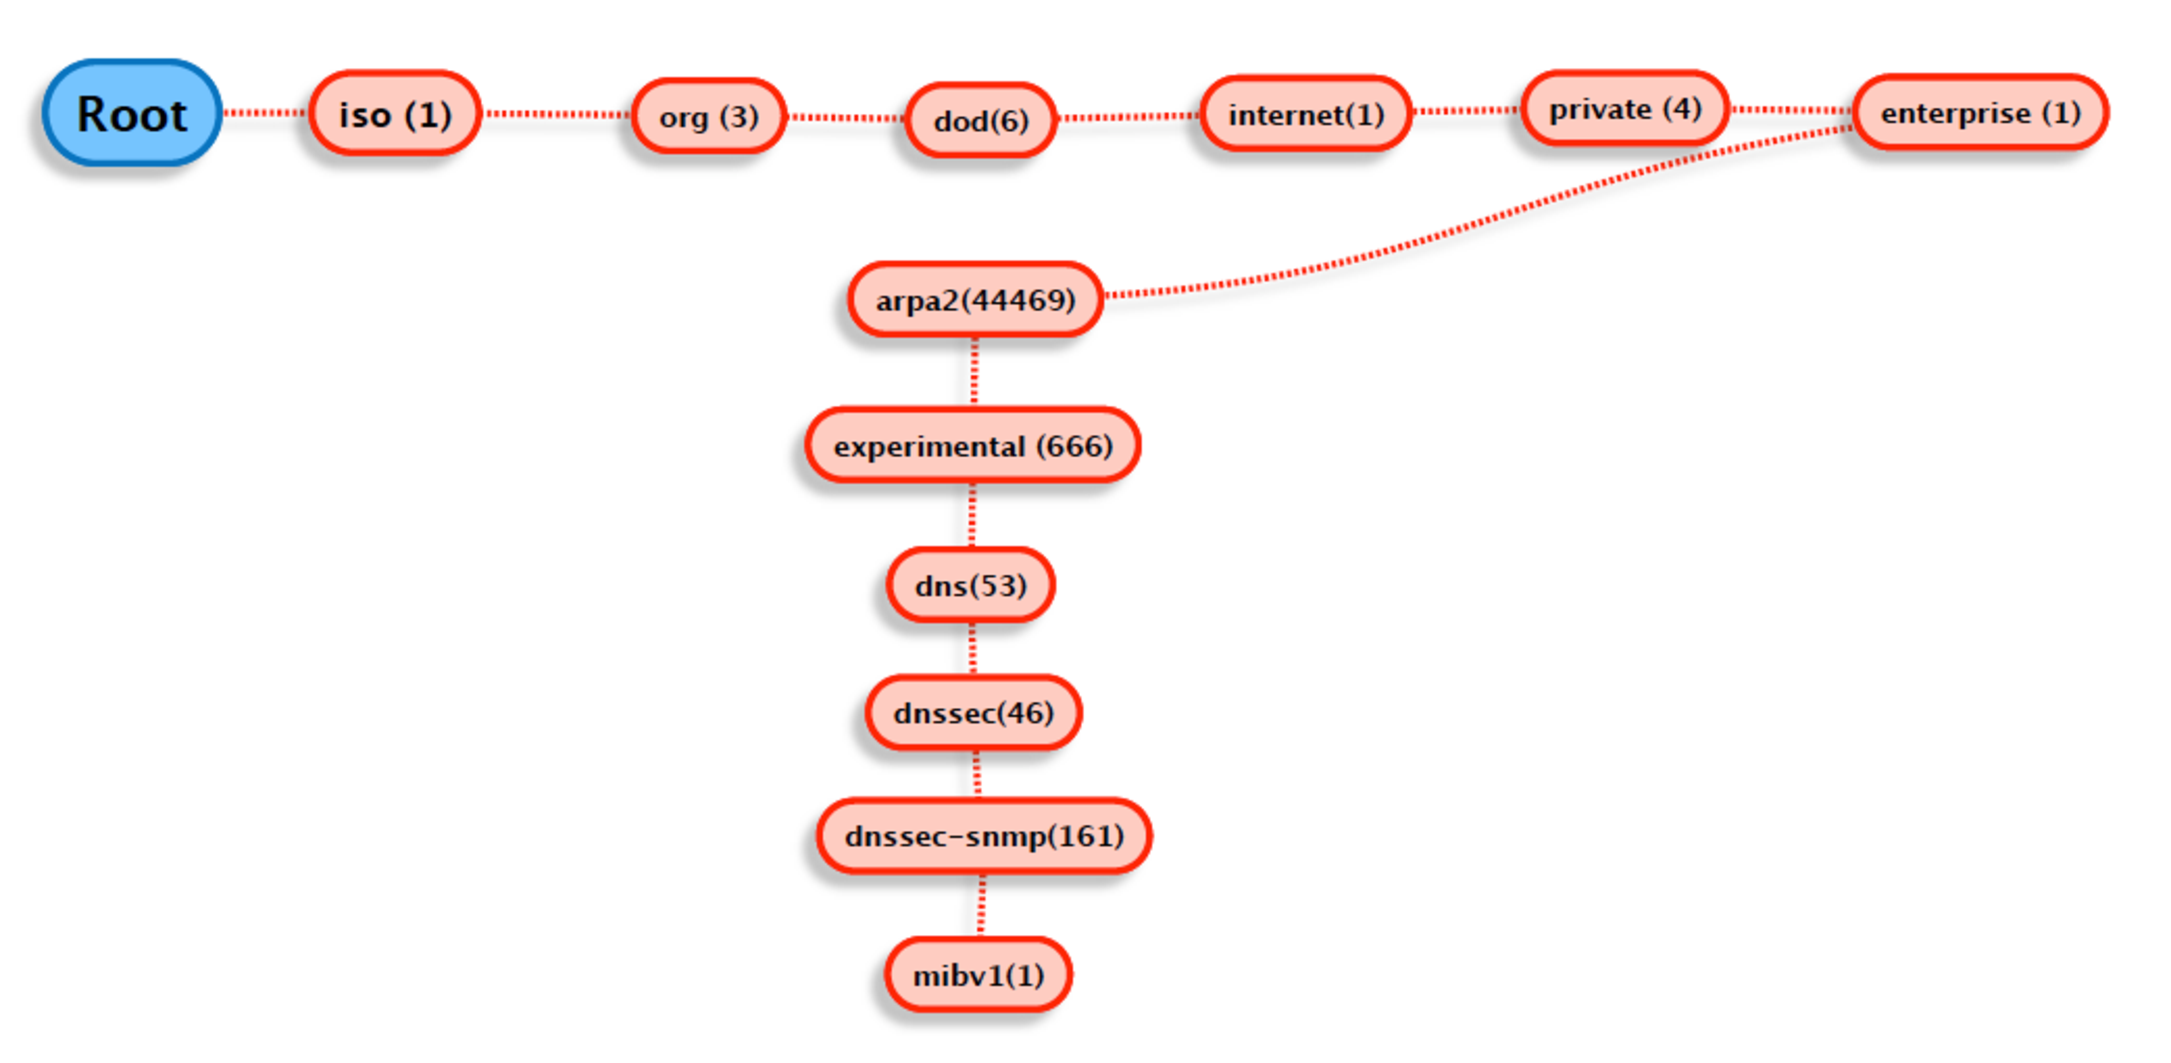
\includegraphics[scale=0.4]{Images/oid-tree.pdf}
\caption{OID Tree}
\label{figure:oid-tree}
\end{figure}


Objects defined in the MIB are organized in tables \footnote{In SNMP terminology, tables are denoted as conceptual tables or columnar objects} or scalar types. INTEGER datatypes are used to represent boolean and numeric values and data type  OCTET-STRING to represent strings (e.g domain names). Four tables are included in the MIB \textit{(dnssecZoneGlobalTable, dnssecZoneAuthNSTable, dnssecZoneSigTable, dnssecZoneDiffTable)}. To provide an easy mechanism to associate data entities to a specific zone, all MIB entries are indexed by the domain name itself (datatype OCTET-STRING).
\\
\subsubsection{Data covered by the MIB}
In section \ref{section:vital-life-signs-dnssec} are listed the most relevant parameters that need to be covered by the MIB, in order to keep track of vital life signs of DNSSEC signed zones. 
\\
The first table \textit{(dnssecZoneGlobalTable)} contains general parameters like the availability of the zone seen from the prospect of an external DNSSEC-aware resolver or the status of the signature verification of the DNSKEY RRset against the published KSK. That table also provides general data like the FQDN of the nameserver, where data is fetched from and its IP address. Furthermore entries in that table supply information about the general DNS setup for a zone. For instance, one could retrieve the information if delegations are present in a zone and subsequently check if the count of DS records matches at least the amount of delegations. 
\\
Entries in table \textit{dnssecZoneGlobalTable} are not supposed to list all data that is provided by the zone. For example, there is no need to list TTL values for each RR when the maximum and minimum TTL observed in a zone is provided. 
\\
The same applies to entries of the \textit{dnssecZoneSigTable}. Only expiration dates of essential RRs at the zone apex are covered, rather than listing each signature expiration date for every RR. For the same reason, entries in the \textit{dnssecZoneDiffTable} only provide a general indication if discrepancies between data provided by a master and slave exist. The perfect candidate to illustrate differences in a master-slave setup is the serial number of the SOA RR itself. The information if a master-slave setup exist for a particular zone can be retrieved from the \textit{dnssecZoneGlobalAuthNSCount} entry in the \textit{ dnssecZoneGlobalTable}.
\\
The general idea of the data provided in all tables in the MIB is to reflect the health status of a zone in a way that it can be easily retrieved from monitoring tools without the need of complex computations.
\\
Listing \ref{lst:snmptranslate} shows all top level elements of the created MIB including tables and their associated indexes.


\begin{listing}
\small\begin{verbatim}

+--arpa2experimentaldnssecMIBv1(1)
   |
   +--dnssecObjects(1)
   |  |
   |  +--dnssecGeneral(1)
   |  |  |
   |  +--dnssecZoneGlobal(2)
   |  |  |
   |  |  +--dnssecZoneGlobalTable(2)
   |  |     |
   |  |     +--dnssecZoneGlobalEntry(1)
   |  |        |  Index: dnssecZoneGlobalIndex
   |  |
   |  +--dnssecZoneAuthNS(3)
   |  |  |
   |  |  +--dnssecZoneAuthNSTable(3)
   |  |     |
   |  |     +--dnssecZoneAuthNSEntry(1)
   |  |        |  Index: dnssecZoneGlobalIndex
   |  |        |
   |  +--dnssecZoneSig(4)
   |  |  |
   |  |  +--dnssecZoneSigTable(4)
   |  |     |
   |  |     +--dnssecZoneSigEntry(1)
   |  |        |  Index: dnssecZoneGlobalIndex
   |  |        |
   |  +--dnssecZoneDiff(5)
   |     |
   |     +--dnssecZoneDiffTable(5)
   |        |
   |        +--dnssecZoneDiffEntry(1)
   |           |  Index: dnssecZoneGlobalIndex
   |           |
   +--dnssecMIBConformance(2)
      |
      +--dnssecMIBGroups(1)
      |  |
      |  +--dnssecMIBScalarGroup(1)
      |  +--dnssecMIBTableGroup(2)
      |
      +--dnssecMIBCompliances(2)


\end{verbatim}
\normalsize
\caption{Structure of ARPA2-Experimental-DNSSEC-MIBv1}
\label{listing:snmptranslate}
\end{listing}  


\subsubsection{Usage of textual conventions and table indexing}

To add more restrictions to the defined object-types and their indexes, textual conventions are used. Figure \ref{figure:textual-conventions} shows the impact of textual conventions for object-type \textit{dnssecZoneGlobalServFail} in table \textit{dnssecZoneGlobalTable} and its representation inside an SNMP packet.    

%%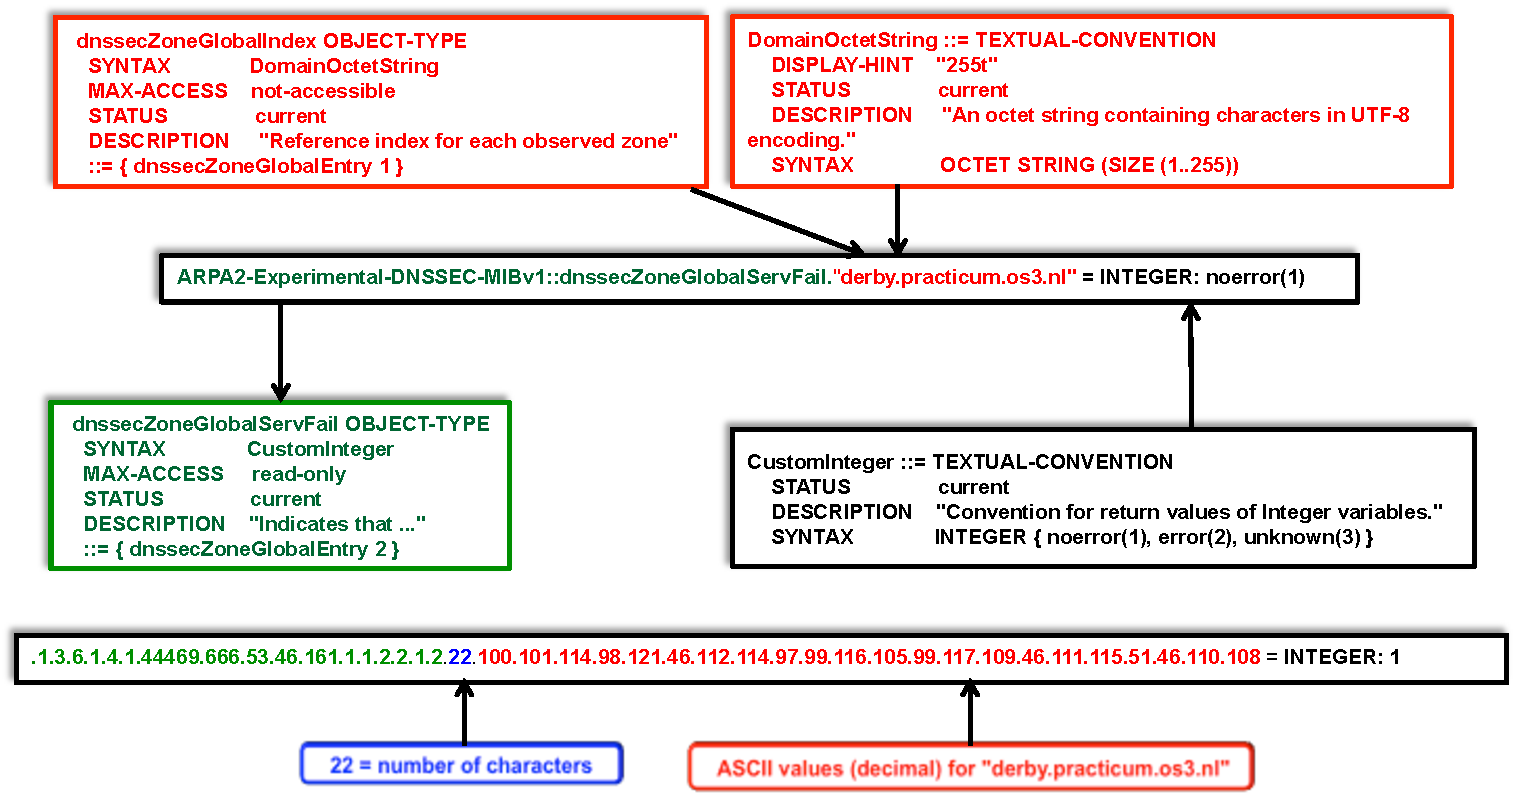
\includepdf[pages=-,scale=.7,pagecommand={}]{Images/tc1.pdf}
%%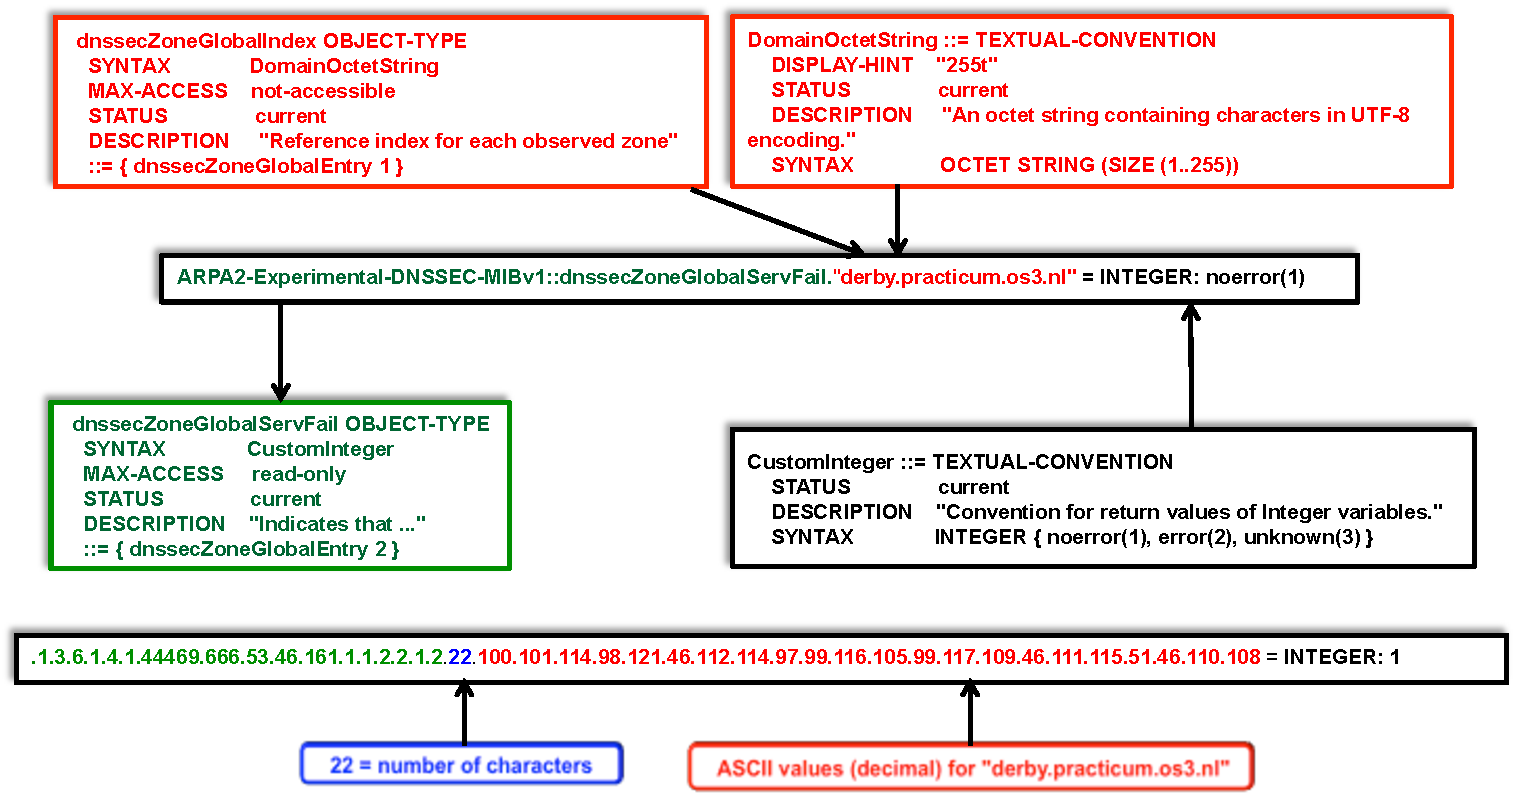
\includepdf[pages={1}]{Images/tc1.pdf}

\begin{figure}[htp] \centering{
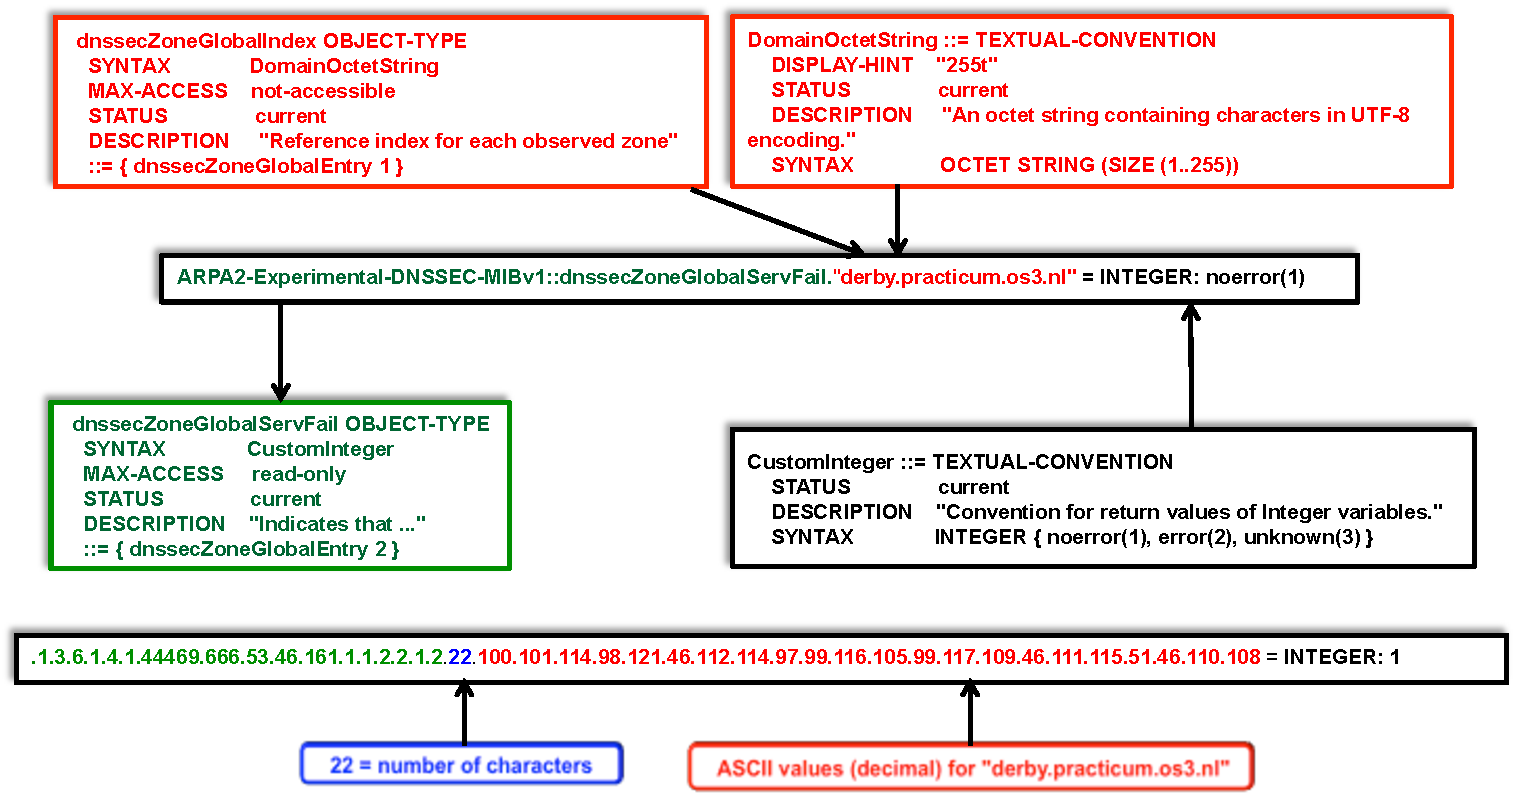
\includegraphics[scale=0.5]{Images/tc1.pdf}}
\caption{Effect of textual conventions to represent MIB data}
\label{figure:textual-conventions}
\end{figure}

A textual convention \textit{DomainOctetString} is defined and mapped to the \textit{dnssecZoneGlobalIndex}. That textual convention specifies the usage of the underlying datatype OCTET STRING and limits its number of octets to 255. That number represents the maximum allowed number of octets a domain name can contain \cite{wiki-domainnames}. Although the maximum allowed number of octets a domain name can contain is limited to 255, an IDNE proposal \cite{idne} (Internationalized domain names using EDNS) exists that uses the DNS extension mechanism called EDNS \cite{edns}. The extension allows some IDNE labels to be longer than 63 characters and some IDNE names to be longer than 255 octets. That would allow to send domain names either as ASCII or binary, and the binary format is UTF-8. The \textit{DISPLAY-HINT} clause specifies the usage of UTF-8 encoded characters \cite{smi-tc}. That string, which represents a domain name is appended as an index value to each instance of an object-type.
\\ 
The textual convention \textit{CustomInteger} restricts the values that object-type \textit{dnssecZoneGlobalServFail} can have. In that case we allow the values shown in table \ref{table-tc}. That enables us to implement our agent data wrapper scripts in a way that for each check only these values can occur and we can associate them to a textual equivalent. Figure \ref{figure:textual-conventions} also shows the numerical representation of an instance of object-type\textit{dnssecZoneGlobalServFail} and how the OID for the SNMP message is constructed on the wire. The green marked numbers are the numerical identifiers for the object-type itself. Then the number of characters of the associated index is appended to the OID and finally the ASCII values in decimal for each character of the domain name. 

\begin{table}[h]
   \centering
  \begin{tabular}{|c|c|}
  \hline
  \textbf{Value} & \textbf{Meaning} \\
  \hline
  1 & No error \\
  \hline
  2 & Error \\
  \hline
  3 & Unknown \\
  \hline  
\end{tabular} 
\caption{Textual convention for integer variables }
\label{table-tc}
\end{table}
 

\subsection{SNMP Subagent implementation}
\label{section:sub-agent-implementation}
The SNMP subagent itself is based on the work of Pieter Hollants \cite{pythonnetsnmpagent} and provides us a Python API to communicate with the NET-SNMP master agent. The main function that updates the defined SNMP objects was implemented during the research project. That function uses the API calls shown in Table \ref{table:api-calls}.

\begin{table}[H]
\begin{tabular}{|l|p{5.5cm}|}
\hline 
\textbf{API call} & \textbf{Description} \\ 
\hline 
tablename.clear & clears a table row\\ 
\hline 
tablename.addRow & adds a table row\\ 
\hline 
tablenamerowid.setRowCell & sets a value to a cell in a table row\\ 
\hline 
\end{tabular} 
\caption{API calls python-netsnmpagent}
\label{table:api-calls}
\end{table}

The values that are assigned to object-type instances are derived from a XML data file. The function that implements the SNMP variables update reads in the XML structure and iterates for all announced zones through the XML document using XPath queries \citep{xpath}. Everytime a corresponding table  entry is identified, that entry and in turn the related SNMP variable gets updated. The function is included in the appendices (TODO). Figure \ref{figure:workflow} shows the  workflow of the function.

\begin{figure}[H]
\centering
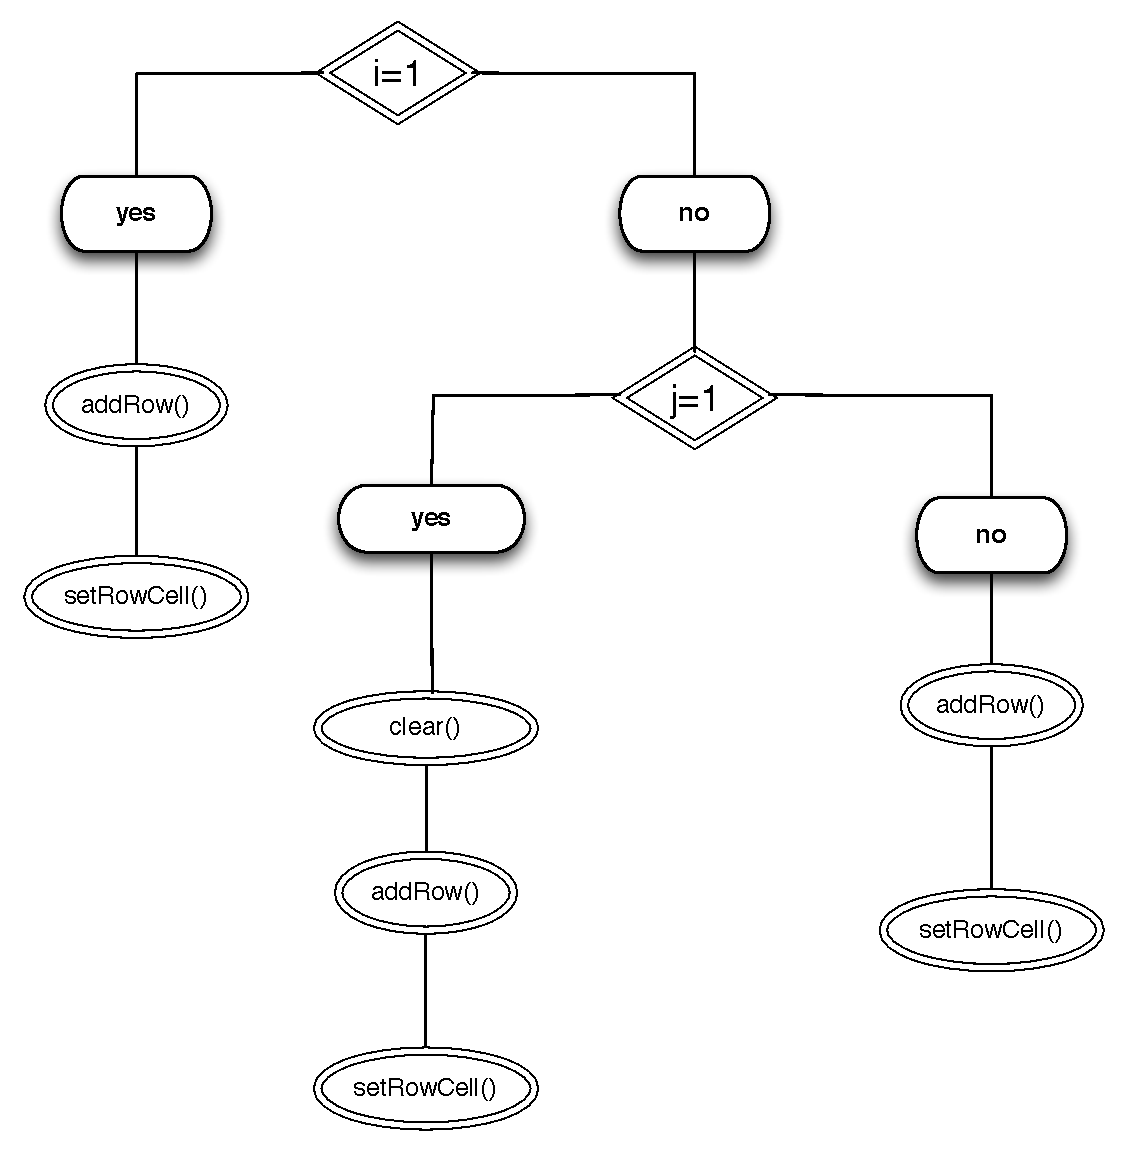
\includegraphics[scale=0.5]{Images/workflow.png}
\caption{workflow of the subagent's UpdateSNMPObjs() function}
\label{figure:workflow}
\end{figure}

The function first checks if it is executed the first time \textit{(i=1)}. If so, table rows are added instantly. The counter variable \textit{i} is increased by one each time the function is called. If \textit{i} is not equal one  another counter variable \textit{j} is checked. That counter indicates which round of iteration is currently performed inside the function. Only, and only if it is the first iteration , the current table is cleared and after that new values are added.
\\
The SNMP subagent operates asynchronously. The data update thread is decoupled from the data providing thread. This ensures periodic data updates and also makes sure that SNMP requests will always be replied to in time. Figure \ref{figure:subagent} shows the interaction between all components that are involved.

\begin{figure}[H]
\centering
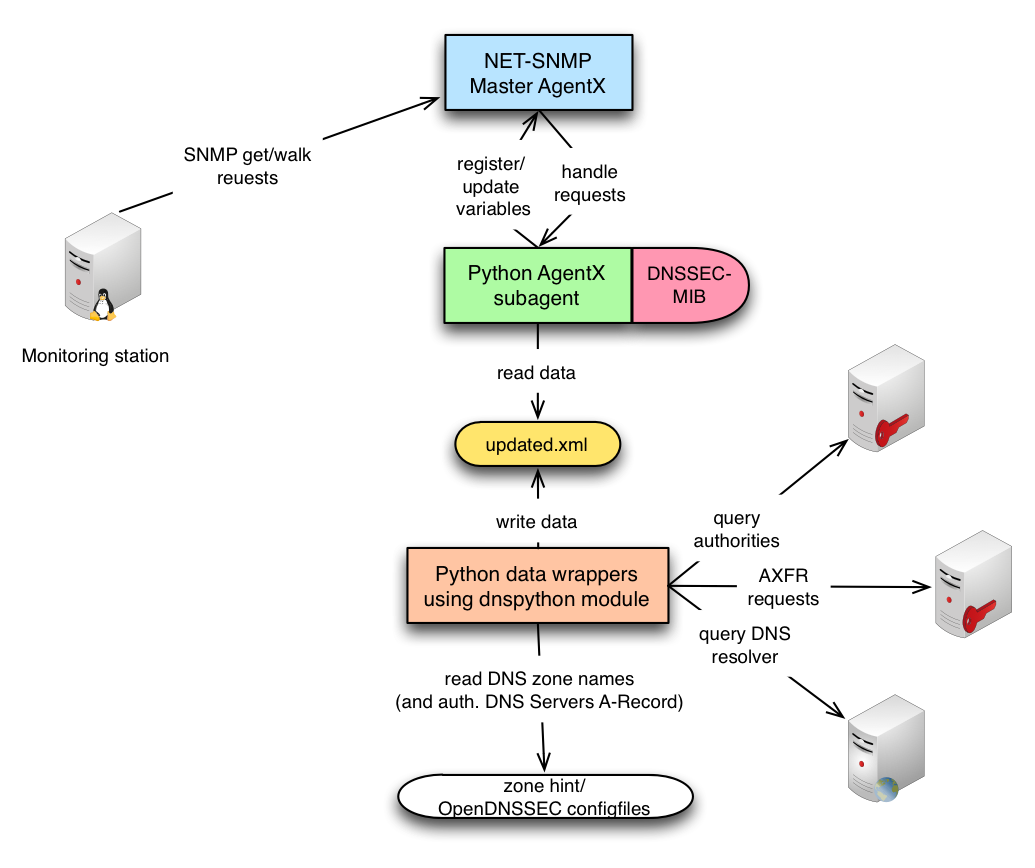
\includegraphics[scale=0.7]{Images/topology3.png}
\caption{logical scheme SNMP subagent}
\label{figure:subagent}
\end{figure}
 

 








\subsection{Conduct DNSSEC monitoring}
\label{section:conduct-dnssec-monitoring}
In order to present how monitoring can be conducted using our created MIB, a use-case example is sketched. To implement the monitoring tasks, the well known monitoring system Nagios \cite{nagios} and its SNMP plugin \textit{check-snmp} \cite{check-snmp} is used.
%%\textit{check_snmp}      %%\cite{check_snmp} is used. 
\\
Let's assume the RRSIG RR of the SOA record and the DNSKEY RR (KSK) of the DNSSEC signed zone \textit{paris.derby.practicum.os3.nl} have expired. That will lead a DNSSEC-aware resolver to invalidate the complete zone. A DNSSEC-aware resolver will only return a SERVFAIL without specifying the root cause for the invalidation when it is queried for RR of that zone. In that case, querying the corresponding OIDs using our MIB might be helpful. Values for the object-type \textit{ dnssecZoneGlobalServFail} will return an error (2) but also the validation check \textit{dnssecZoneGlobalDNSKEYSignatureVerification} in table \textit{dnssecZoneGlobalTable} will return an error (2) for that zone. 
\\
The actual reason for the SERVFAIL can be derived from table \textit{ dnssecZoneSigTable}, in particular from object-type \textit{ dnssecZoneSigDNSKEYSignatureExpirationTime}. It will show an expired date for that RRSIG RR, in that case the expiration of the RRSIG occurred on 27th of January 2015 at 19:50:10. Figure \ref{figure:nagios} shows the applied Nagios implementation.

\begin{figure}[H]
\centering
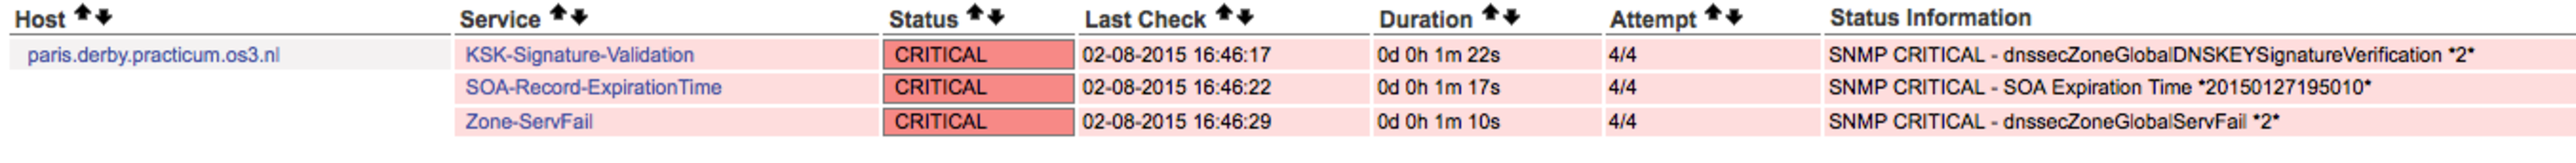
\includegraphics[scale=0.3]{Images/nagios.pdf}
\caption{implemented Nagios checks based on values of the DNSSEC-MIB}
\label{figure:nagios}
\end{figure}



\newpage

\section{Conclusion}
\label{chap:conclusion}

Build a proof of concept and conduct monitoring based on that concept. We implemented all components (Agent, SNMP MIB, Data collection ...)




\newpage

\section{Future work}
\label{chap:future-work}
What checks/variables could be added to MIB:
validate all RRSIGs and return number of validated/ non validated

compare DS record in parent zone against proposed DNSKEY in child zone

SNMP traps / notifications

IDN / Punny code implementation

NSEC(3) checks (see validns)





\newpage

\section*{Acknowledgments}
\addcontentsline{toc}{section}{Acknowledgement}
\label{chap:acknowledgments}

\newpage

\section*{References}
\addcontentsline{toc}{section}{References}
\label{chap:references}
\begin{thebibliography}{99}
\bibitem{stats} ICANN, {\em TLD statistics regarding DNSSEC}, January 2014, \url{http://stats.research.icann.org/dns/tld_report/}
\bibitem{list} Dagmar Hilmarsdottir, {\em not exhaustive list of DNSSEC monitoring tools}, May 2011, \url{info.menandmice.com/blog/bid/58099/DNSSEC-monitoring-tools}
\bibitem{pythonnetsnmpagent} Pieter Hollants, {\em Python-netsnmpagent Module}, 2013, \url{https://github.com/pief/python-netsnmpagent}
\bibitem{dnsmib} R. Austein \& J. Saperia, {\em DNS Server MIB Extensions}, May 1994, \url{https://tools.ietf.org/html/rfc1611}
\bibitem{dnsmib_retire} R. Austein, {\em Applicability Statement for DNS MIB Extensions}, November 2001, \url{https://tools.ietf.org/html/rfc3197}
\bibitem{snmp-rfc} SNMP RFC, {\em Overview of SNMP related RFC's}, 2013 \url{http://www.snmp.com/protocol/snmp_rfcs.shtml} 
\bibitem{agentx} RFC2741,  {\em Agent Extensibility (AgentX) Protocol}, January 2000, \url{https://www.ietf.org/rfc/rfc2741.txt}
\bibitem{smiv2} RFC2578, {\em Structure of Management Information Version 2 (SMIv2)}, April 1999, \url{https://tools.ietf.org/html/rfc2578}
\bibitem{smi-tc} RFC2579, {\em Textual Conventions for SMIv2}, April 1999, \url{https://tools.ietf.org/html/rfc2579}
\bibitem{cisco-snmp} William Stallings (Cisco Systems, Inc), {\em Security Comes to SNMP: The New SNMPv3 Proposed Internet Standards}, January  2015, \url{http://www.cisco.com/web/about/ac123/ac147/archived_issues/ipj_1-3/snmpv3.html}
\bibitem{oid1} OID repository, {\em iso(1) identified-organization(3) dod(6) internet(1)}, October 2013, \url{http://oid-info.com/get/1.3.6.1}
\bibitem{perkins} T. Perkins, {\em Understanding SNMP MIBs Revision 1.1.7 },September 1993, \url{http://www.dsc.ufcg.edu.br/~jacques/cursos/gr/recursos/outros/perkins.pdf}
\bibitem{net-snmp} NET-SNMP, {\em Suite of applications used to implement SNMP}, February 2013, \url{http://www.net-snmp.org/}
\bibitem{agentx-netsnmp} NET-SNMP, {\em AgentX extension for NET-SNMP}, May 2011, \url{http://www.net-snmp.org/docs/README.agentx.html}
\bibitem{dnspython} dnspython, {\em DNS toolkit for Python}, September 2013, \url{http://www.dnspython.org/}
\bibitem{dig} dig, {\em DNS lookup utility and part of the BIND domain name server software suite}, unknown, \url{ftp://ftp.isc.org/isc/bind9/cur/9.10/doc/arm/man.dig.html}
\bibitem{validns} validns, {\em DNS/DNSSEC zone validator}, 2012, \url{http://www.validns.net/}
\bibitem{rfc_dnssec} D. Eastlake \& C. Kaufman, {\em First DNSSEC specifications}, January 1997, \url{http://www.ietf.org/rfc/rfc2065.txt}
\bibitem{et} Python Software Foundation, {\em The ElementTree XML API}, 01 January 2015, \url{https://docs.python.org/2/library/xml.etree.elementtree.html}
\bibitem{snmp-wire} Rane Corporation, {\em SNMP: Simple? Network Management Protocol}, December  2005, \url{http://www.rane.com/note161.html}
\bibitem{ber-asn1} ITU-T Recommendation X.690 , {\em ASN.1 encoding rules}, July 2002, \url{http://www.itu.int/ITU-T/studygroups/com17/languages/X.690-0207.pdf}
\bibitem{wiki-domainnames} Wikipedia, {\em Domain Name System}, February  2015, \url{http://en.wikipedia.org/wiki9/Domain_Name_System#Domain_name_syntax}
\bibitem{xpath} Python Software Foundation, {\em XPath Support}, January  2015, \url{https://docs.python.org/2/library/xml.etree.elementtree.html#elementtree-xpath}
\end{thebibliography}


%%\section*{Appendices}
\addcontentsline{toc}{section}{Appendices}
\label{chap:appendices}
\end{document}
